% --- Template for thesis / report with tktltiki2 class ---
% 
% last updated 2013/02/15 for tkltiki2 v1.02

\documentclass[english]{tktltiki2}

% tktltiki2 automatically loads babel, so you can simply
% give the language parameter (e.g. finnish, swedish, english, british) as
% a parameter for the class: \documentclass[finnish]{tktltiki2}.
% The information on title and abstract is generated automatically depending on
% the language, see below if you need to change any of these manually.
% 
% Class options:
% - grading                 -- Print labels for grading information on the front page.
% - disablelastpagecounter  -- Disables the automatic generation of page number information
%                              in the abstract. See also \numberofpagesinformation{} command below.
%
% The class also respects the following options of article class:
%   10pt, 11pt, 12pt, final, draft, oneside, twoside,
%   openright, openany, onecolumn, twocolumn, leqno, fleqn
%
% The default font size is 11pt. The paper size used is A4, other sizes are not supported.
%
% rubber: module pdftex

% --- General packages ---

\usepackage[utf8]{inputenc}
\usepackage[T1]{fontenc}
\usepackage{lmodern}
\usepackage{microtype}
\usepackage{amsfonts,amsmath,amssymb,amsthm,booktabs,color,enumitem,graphicx}
\usepackage[pdftex,hidelinks]{hyperref}
\usepackage[ruled,vlined,linesnumbered]{algorithm2e}
\usepackage{caption}
\usepackage{float}
\usepackage{subcaption}
\usepackage{pdfpages}

% Algorithm2e environment with "Algoritmi"-caption.
%\newenvironment{finalgo}[1][htb]{
%  \renewcommand{\algorithmcfname}{Algoritmi}
%  \begin{algorithm}[#1]
%}{\end{algorithm}}

% To be able to not numbering individual lines:
\let\oldnl\nl% Store \nl in \oldnl
\newcommand{\nonl}{\renewcommand{\nl}{\let\nl\oldnl}}

% Automatically set the PDF metadata fields
\makeatletter
\AtBeginDocument{\hypersetup{pdftitle = {\@title}, pdfauthor = {\@author}}}
\makeatother

% --- Language-related settings ---
%
% these should be modified according to your language

% babelbib for non-english bibliography using bibtex
\usepackage[fixlanguage]{babelbib}
\selectbiblanguage{english}

% add bibliography to the table of contents
\usepackage[nottoc]{tocbibind}
% tocbibind renames the bibliography, use the following to change it back
\settocbibname{References}

%%%%%%%%%%%%% Algorithm2e %%%%%%%%%%%%%
\SetKw{KwOutput}{output}
\SetKw{KwNotMapped}{is not mapped in }
%%%%%%%%%%%%%%%%%%%%%%%%%%%%%%%%%%%%%%%

% --- Theorem environment definitions ---
\newtheorem{mythm}{Theorem}[section]
\newtheorem{mylem}[mythm]{Lemma}
\newtheorem{mycor}[mythm]{Corollary}

\theoremstyle{definition}
\newtheorem{mydef}[mythm]{Definition}
\newtheorem{alg}[mythm]{Algoritmi}
\newtheorem{esim}[mythm]{Example}

\theoremstyle{remark}
\newtheorem*{huom}{Huomautus}

\DeclareMathOperator*{\argmin}{arg\, min}

% --- tktltiki2 options ---
%
% The following commands define the information used to generate title and
% abstract pages. The following entries should be always specified:

\title{Title will be here}
\author{Rodion Efremov}
\date{\today}
\level{Master thesis}
\abstract{Abstract goes here}

\keywords{}

% classification according to ACM Computing Classification System (http://www.acm.org/about/class/)
% This is probably mostly relevant for computer scientists
% uncomment the following; contents of \classification will be printed under the abstract with a title
% "ACM Computing Classification System (CCS):"
% \classification{}

% If the automatic page number counting is not working as desired in your case,
% uncomment the following to manually set the number of pages displayed in the abstract page:
%
% \numberofpagesinformation{16 sivua + 10 sivua liitteissä}
%
% If you are not a computer scientist, you will want to uncomment the following by hand and specify
% your department, faculty and subject by hand:
%
% \faculty{Matemaattis-luonnontieteellinen}
% \department{Tietojenkäsittelytieteen laitos}
% \subject{Tietojenkäsittelytiede}
%
% If you are not from the University of Helsinki, then you will most likely want to set these also:
%
% \university{Helsingin Yliopisto}
% \universitylong{HELSINGIN YLIOPISTO --- HELSINGFORS UNIVERSITET --- UNIVERSITY OF HELSINKI} % displayed on the top of the abstract page
% \city{Helsinki}
%


\begin{document}

% --- Front matter ---

\frontmatter      % roman page numbering for front matter

\maketitle        % title page
\makeabstract     % abstract page

\tableofcontents  % table of contents

% --- Main matter ---

\mainmatter       % clear page, start arabic page numbering

% --- References ---
%
% bibtex is used to generate the bibliography. The babplain style
% will generate numeric references (e.g. [1]) appropriate for theoretical
% computer science. If you need alphanumeric references (e.g [Tur90]), use
%
% \bibliographystyle{babalpha-lf}
%
% instead.

\section*{Dummy section}

\subsection{Strongly connected components}
Since our methods require the input graph to be strongly connected, we review here briefly how to algorithmically validate that the input graph exhibits the requirement. A strongly connected component is any (maximal) subset of vertices $C$, such that any node $u \in C$ is reachable from any other node of $C$. A directed graph $G = (V, A)$ is called \textit{strongly connected} if and only if $V$ is a strongly connected component.

We say that $u$ and $v$ are \textit{mutually reachable} whenever they are reachable from each other. Let $u \overset{r}{\sim} v$ denote the aforementioned reachability relation. Now, it is easy to see that
\begin{description}
\item[\textsc{(Reflexivity)}]  $u \overset{r}{\sim} u$, for all $u \in V(G)$.
\item[\textsc{(Symmetry)}] if  $u \overset{r}{\sim} v$, then $v \overset{r}{\sim} u$.
\item[\textsc{(Transitivity)}] If $u \overset{r}{\sim} v$ and $v \overset{r}{\sim} v'$, then $u \overset{r}{\sim} v'$.
\end{description}
The above three properties imply that $\overset{r}{\sim}$ is an equivalence relation, and as such, implies that the graph has a unique partition into strongly connected components. Note that any node is contained within exactly one strongly connected component.

Algorithms for finding all strongly connected components of a graph in linear time are known. We review three of them below.

\subsubsection{Kosaraju's algorithm}

% DEFINITION: Graph transpose
\begin{mydef}
Given a directed graph $G = (V, A)$, the \textit{transpose} of $G$ is the graph $G^T = (V, A^T)$, where $A^T = \{ (v, u) \colon (u, v) \in A \}$.
\end{mydef}

% THEOREM: Graph and its transpose have same SCC
\begin{mythm}
Any directed graph $G = (V,A)$ has exactly the same strongly connected components as its transpose $G^T = (V, A^T)$.

\begin{proof}
Let $u, v \in V$ be two distinct nodes of the graph. We need to show that $u$ and $v$ are mutually reachable in $G$ if and only if they are mutually reachable in the transpose graph $G^T$. Suppose $u$ and $v$ are mutually reachable in $G$. Now, there are two distinct paths: $\pi_{uv}$ is an $u-v$ path, and $\pi_{vu}$ is a $v-u$ path. Taking the transpose of the graph (changing the direction of each arc), $\pi_{uv}$ becomes a $v-u$ path, and $\pi_{vu}$ becomes a $u-v$ path. Hence, the two nodes $u$ and $v$ are mutually reachable also in the transpose graph. 

Suppose now that $u$ and $v$ are not mutually reachable. This implies that there may exist a $u-v$ path $\pi_{uv}$, or a $v-u$ path $\pi_{vu}$, but not both. Assume that only $\pi_{uv}$ exists. Now, in the transpose graph, there is a $v-u$ path, yet no $v-u$ path, and so $u$ and $v$ are not mutually reachable in the transpose. The case of $\pi_{vu}$ is symmetrical. 

Since we assumed the nodes $u$ and $v$ to be arbitrary, the result follows.
\end{proof}
\end{mythm}

Kosaraju's algorithm sacrifices two depth-first search traversals over the input graph: the first one in forward direction and the second one in backward direction (from a node to its parents). As such, it relies on the fact that any directed graph $G$ has exaclty the same strongly connected components than its transpose $G^T$, and uses that observation for detecting strongly connected components.

% ALGORITHM: KosarajuVisit
\begin{algorithm}
\If{$v \not \in S$}{
  $S \leftarrow S \cup \{ v \}$ \\
  \ForEach{$(v, w) \in G(A)$}{
     \textsc{KosarajuVisit}$(G, S, L, w)$ \\
  }
  
  $L \leftarrow \langle v \rangle \circ L$ \\
}
\caption{\textsc{KosarajuVisit}$(G, S, L, v)$}
\label{alg:kosaraju_visit}
\end{algorithm}

% ALGORITHM: KosarajuAssign
\begin{algorithm}
\If{$u$ \KwNotMapped $\mu$}{
  $\mu(u) \leftarrow r$ \\
  \nonl For all parents of $u$ \\
  \ForEach{$(v, u) \in G(A)$}{
    \textsc{KosarajuAssign}$(G, \mu, v, r)$ \\
  }
}
\caption{\textsc{KosarajuAssign}$(G, \mu, u, r)$}
\label{alg:kosaraju_assign}
\end{algorithm}

% ALGORITHM: KosarajuSCC
\begin{algorithm}
$S \leftarrow \varnothing$ \\
$L \leftarrow \langle \rangle$ \\
$\mu \leftarrow \varnothing$ \\
\ForEach{$v \in V(G)$}{
  \textsc{KosarajuVisit}$(G, S, L, v)$ \\
}
\nonl Iterate the list $L$ in its natural order \\
\ForEach{$v \in L$}{
  \textsc{KosarajuAssign}$(G, \mu, v, v)$ \\
}
$f = \varnothing$ \\
\ForEach{$(v, i) \in \mu$}{
  \If{$i$ \KwNotMapped $f$}{
    $f(i) \leftarrow \{ v \}$ \\
  } 
  \Else{
    $f(i) \leftarrow f(i) \cup \{ v \}$ \\
  }
}
\ForEach{$(i \mapsto C) \in f$}{
  \KwOutput $C$ \\
}
\caption{\textsc{KosarajuSCC}$(G)$}
\label{alg:kosaraju}
\end{algorithm}

\subsubsection{Tarjan's algorithm}
Tarjan's algorithm (\cite{Tarjan1971}) for strongly connected components achieves better running times than Kosaraju's algorithm despite the fact that the former was discovered prior to the latter. It does so by doing only one depth-first traversal over the graph, unlike the Kosaraju's algorithm that requires two.

% ALGORITHM: TarjanStrongConnect
\begin{algorithm}
$i(u) \leftarrow j$ \\
$l(u) \leftarrow j$ \\
$j \leftarrow j + 1$ \\
$\textsc{Push}(S, u)$ \\
\ForEach{$(u, v) \in G(A)$}{
  \If{$v$ \KwNotMapped $i$}{
    \textsc{TarjanStrongConnect}$(G, v, i, l, j, S)$ \\
    $l(u) \leftarrow \min(l(u), l(v))$ \\
  } 
  \ElseIf{$v \in S$}{
    $l(u) \leftarrow \min(l(u), i(v))$ \\
  }
}
\If{$l(u) = i(u)$}{
  $C = \varnothing$ \\
  \Repeat{$w \neq u$}{
    $w = \textsc{Pop}(S)$ \\
  	$C \leftarrow C \cup \{ w \}$ \\
  	}
  \KwOutput $C$ \\
}
\caption{\textsc{TarjanStrongConnect}$(G, u, i, l, j, S)$}
\label{alg:tarjan_strong_connect}
\end{algorithm}

% ALGORITHM: TarjanSCC
\begin{algorithm}
$S \leftarrow \varnothing$ \\
$i \leftarrow \varnothing$ \\
$l \leftarrow \varnothing$ \\
$j \leftarrow 0$ \\
\ForEach{$u \in G(V)$}{
  \If{$u$ \KwNotMapped $i$}{
    \textsc{TarjanStrongConnect}$(G, u, i, l, j, S)$ \\
  }
}
\caption{\textsc{TarjanSCC}$(G)$}
\label{alg:tarjan}
\end{algorithm}

\subsubsection{Path-based algorithm}
What comes to path-based strongly connected component algorithms, there are several version of the algorithm, with some of them running in superlinear time. The following algorihtm is due to Gabow \cite{Gabow2000}:

% ALGORITHM: GabowVisit
\begin{algorithm}
$\pi(u) \leftarrow c$ \\
$c \leftarrow c + 1$ \\
$S \leftarrow S \cup \{ u \}$ \\
$P \leftarrow P \cup \{ u \}$ \\
\ForEach{$(u, v) \in G(A)$}{
  \If{$v$ \KwNotMapped $\pi$}{
     \textsc{GabowVisit}$(G, v, c, \pi, S, P, A)$ \\
  }
  \ElseIf{$v \not \in A$}{
    \While{$\pi(\textsc{Top}(P)) > \pi(v)$}{
      \textsc{Pop}$(P)$ \\
    }
  }
}
\If{$u = \textsc{Top}(P)$}{
  \textsc{Pop}$(P)$ \\
  $C \leftarrow \varnothing$ \\
  \Repeat{\textsc{Top}$(S) \neq u$}{
    $w \leftarrow \textsc{Pop}(S)$ \\
    $A \leftarrow A \cup \{ w \}$ \\
    $C \leftarrow C \cup \{ c \}$ \\
  }
  \KwOutput $C$ \\
}
\caption{\textsc{GabowVisit}$(G, u, c, \pi, S, P, A)$}
\label{alg:gabowvisit}
\end{algorithm}

% ALGORITHM: GabowSCC
\begin{algorithm}
$S \leftarrow \varnothing$ \\
$P \leftarrow \varnothing$ \\
$A \leftarrow \varnothing$ \\
$\pi \leftarrow \varnothing$ \\
$c \leftarrow 0$ \\
\ForEach{$u \in V(G)$}{
  \If{$u$ \KwNotMapped $\pi$}{
    \textsc{GabowVisit}$(G, u, c, \pi, S, P, A)$ \\
  }
}
\caption{\textsc{GabowSCC}$(G)$}
\label{alg:gabow}
\end{algorithm}

\subsubsection{Comparing the algorithms}
\begin{figure}
  \centering
  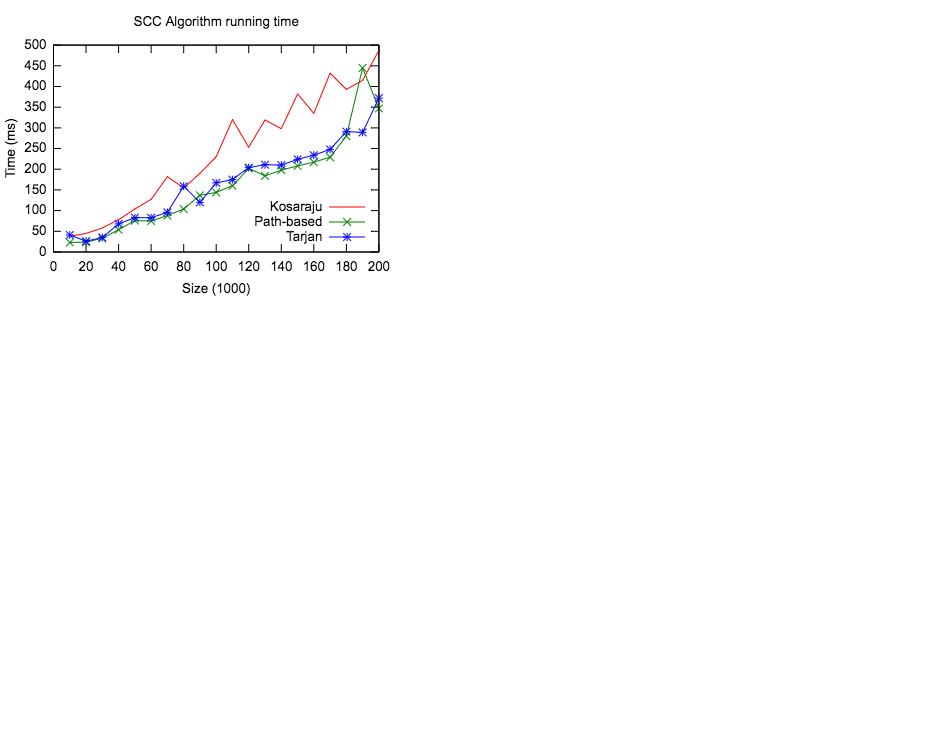
\includegraphics[width=600px,height=500px,keepaspectratio,trim=10 200 200 10]{SCCAlgorithmPerformanceFigure}
  \caption{Running times of the strongly connected component algorithms}
\end{figure}

\bibliographystyle{babplain-lf}
\bibliography{refs}


% --- Appendices ---

% uncomment the following

% \newpage
% \appendix
% 
% \section{Esimerkkiliite}

\end{document}